%
% File emnlp2019.tex
%
%% Based on the style files for ACL 2019, which were
%% Based on the style files for EMNLP 2018, which were
%% Based on the style files for ACL 2018, which were
%% Based on the style files for ACL-2015, with some improvements
%%  taken from the NAACL-2016 style
%% Based on the style files for ACL-2014, which were, in turn,
%% based on ACL-2013, ACL-2012, ACL-2011, ACL-2010, ACL-IJCNLP-2009,
%% EACL-2009, IJCNLP-2008...
%% Based on the style files for EACL 2006 by 
%%e.agirre@ehu.es or Sergi.Balari@uab.es
%% and that of ACL 08 by Joakim Nivre and Noah Smith

\documentclass[11pt,a4paper]{article}
\usepackage[hyperref]{emnlp-ijcnlp-2019}
\usepackage{times}
\usepackage{latexsym}

\usepackage{url}

\usepackage{framed}
\usepackage[framemethod=tikz,xcolor=true]{mdframed}
\usepackage{latexsym}
\usepackage{graphicx}
\usepackage[normalem]{ulem}
\usepackage{url}
\usepackage{bm}
\usepackage{booktabs}

\definecolor{t1}{rgb}{.796,.255,.329}
\definecolor{t2}{rgb}{.255, .329, .796}

\aclfinalcopy % Uncomment this line for the final submission

%\setlength\titlebox{5cm}
% You can expand the titlebox if you need extra space
% to show all the authors. Please do not make the titlebox
% smaller than 5cm (the original size); we will check this
% in the camera-ready version and ask you to change it back.
\newcommand\Agolo{\dagger}
\newcommand\CICS{\star}

\newcommand\BibTeX{B{\sc ib}\TeX}
\newcommand\confname{EMNLP-IJCNLP 2019}
\newcommand\conforg{SIGDAT}

\title{Summarizing Relationships for Interactive Concept Map Browsers}

\author{Abram Handler,$^{\CICS}$ Prem Ganeshkumar,$^{\Agolo}$ Brendan O'Connor$^{\CICS}$ and Mohamed AlTantawy$^{\Agolo}$ \\ \\
Agolo$^{\Agolo}$ \\ 
 New York, NY \\ \\
  College of Information and Computer Sciences$^{\CICS}$ \\
  University of Massachusetts, Amherst \\
  {\tt ahandler@cs.umass.edu} \\}

\date{}

\begin{document}
\maketitle

%- We address the problem of how to summarize a relationship in response to a user's query in a concept map interface. 
%- We extend existing work on concept map generation and relationship summarization.
%- We present a model, trained on a new dataset collected for this task. 
%- We release the dataset for future work.


\maketitle\begin{abstract}
Concept maps are visual summaries, structured as directed graphs: important concepts from a dataset are displayed as vertexes, and edges between vertexes show natural language descriptions of the relationships between the concepts on the map. Thus far, preliminary attempts at automatically creating concept maps have focused on building static summaries. However, in interactive settings, users will need to dynamically investigate particular relationships between pairs of concepts. For instance, a historian using a concept map browser might decide to investigate the relationship between two politicians in a news archive. We present a model which responds to such queries by returning one or more short, importance-ranked, natural language descriptions of the relationship between two requested concepts, for display in a visual interface. Our model is trained on a new public dataset, collected for this task.

Code and data are available at:\\ \url{https://github.com/slanglab/ concept_maps_newsum19}
\end{abstract}


\section{Introduction}

Concept maps are visual summaries, structured as directed graphs (Figure \ref{f:map}). Important concepts from a corpus are shown as vertexes. Natural language descriptions of the relationships between concepts are shown as textual labels, along the edges on the map. Initial attempts to generate English-language concept maps within natural language processing \cite{emnlp2017conceptmaps} have focused on creating static diagrams which summarize collections of documents.

\begin{figure}[htb!]
\centering
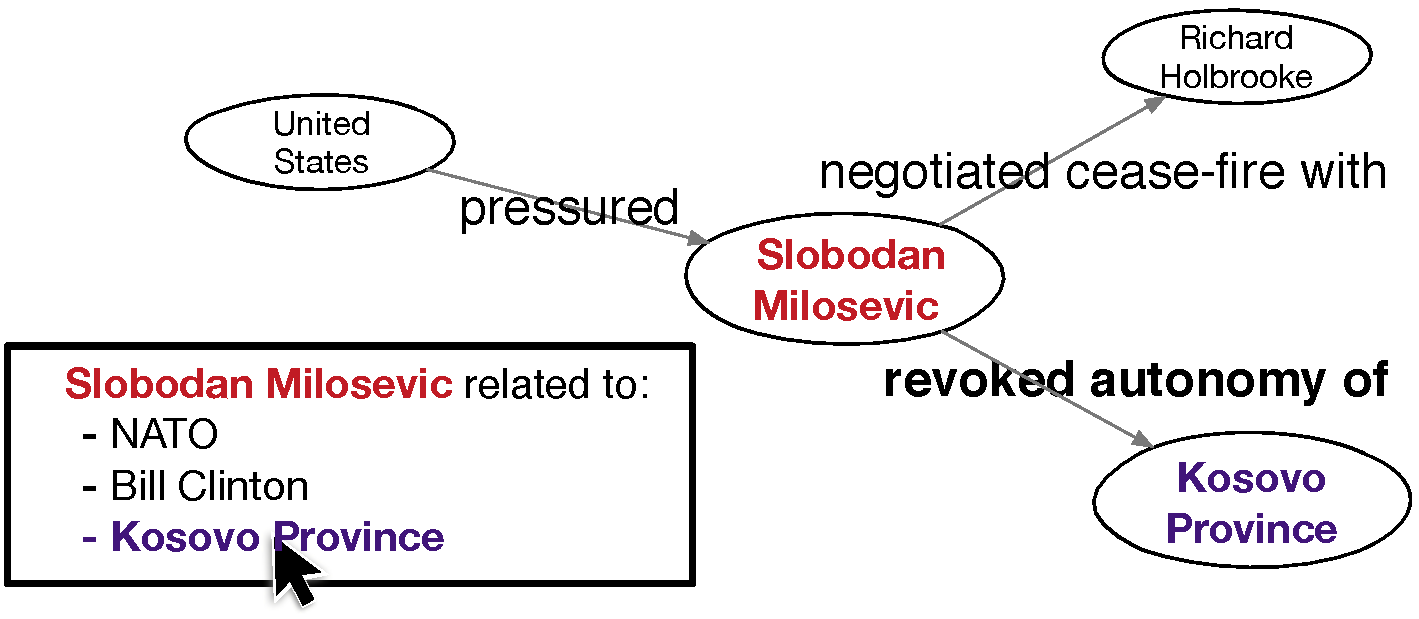
\includegraphics[width=6.5cm]{simple.pdf}
\caption{An example concept map browser. The system indicates that $(t_1)$=``Slobodan Milosevic" is related to $(t_2)$=``Kosovo Province.'' The user clicks to investigate the relationship, and the system must generate a summary explaining how Milosevic is related to Kosovo.}
\label{f:map}
\end{figure}

However, in interactive settings, users will want to query relationships with a concept map interface, rather than simply read over fixed output from a summarization system. For instance, in the concept map browser shown in Figure \ref{f:map}, a user has queried for the relationship between Milosevic and Kosovo. An interactive system should include both concepts in a visual network, along with a labeled edge that summarizes their relationship (e.g. ``Slobodan Milosevic revoked autonomy of Kosovo Province'').

This study is concerned with how to add such labeled summary edges to a map. Given a pair of input query concepts, denoted $(t_1)$ and $(t_2)$, we attempt to select the best extractive, natural language \textit{summary statement} which summarizes their relationship. Because there is no existing supervision to guide such a selection, we collect a new dataset of annotated summary statements, which we use to supervise a new model for this task. 

Our study thus presents a full system for summarizing the relationship between an arbitrary pair of query concepts, extending prior work on relational summarization and concept maps \cite{emnlp2017conceptmaps,N18-1159}.

\section{Related work: relationship extraction}

This study builds on prior efforts from \citet{N18-1159}, who propose extractively summarizing relationships via a two-stage process that first (1) identifies wellformed spans from a corpus that start with $(t_1)$ and end with $(t_2)$ and then (2) chooses the best summary statement from among these wellformed candidates. \citet{N18-1159} show that extracting wellformed spans can find many more readable candidates than traditional relation extraction techniques. But they do not offer a method for the second step of picking a summary statement, which is the focus of this study.

We approach this new task of choosing the best summary statement from available candidates by collecting new supervision, tailored to the particular problem of summarizing relationships on concept maps. This form of supervision has a different focus from the existing \citet{emnlp2017conceptmaps} concept map dataset. Where \citet{emnlp2017conceptmaps} seek to create the best overall concept map for a given \textit{topic}, this work seeks to find the best summary relationship for a given \textit{relationship}. Therefore, unlike  \citet{emnlp2017conceptmaps}, our dataset includes labels for the most readable and informative statement describing the relationship between a $(t_1)-(t_2)$ query pair. 


\section{Overall technical approach}\label{s:approach}

Like \citet{N18-1159}, we approach the problem of finding a short relationship \textit{summary statement} with a two-stage approach. 

\underline{Stage 1:} We identify candidate summary statements using \citet{N18-1159}'s method, which returns the probability that a span of tokens beginning with $(t_1)$ and ending with $(t_2)$ reads as a fluid and coherent sentence when extracted from naturally-occurring text.\footnote{We also allow statements which begin with $(t_2)$ and end with $(t_1)$; the order of query concepts is important in interfaces which display concept maps, but beyond the scope of this work. We limit statements to a max. of 75 characters.}\ (For brevity, we refer the reader to prior work for details, including discussion of why span extraction is preferred to relation extraction techniques). Table \ref{t:spans} provides examples of spans that do and do not make sense when extracted in this manner. We define all spans between $(t_1)$ and $(t_2)$ with a probability of well-formedness greater than .5 to be the \textbf{candidate set} for the pair $(t_1)$ -- $(t_2)$. A sample candidate set is shown in Table \ref{t:matrix}. 

 \begin{table}[htbp!]
% \begin{mdframed}[
%    tikzsetting={draw=black},
%    ]
\begin{tabular}{p{7.1cm}}  \toprule % \toprule
Milosevic withdrew from Kosovo \sout{in 1999}.\\ 
\sout{Clinton spoke with} Milosevic about Kosovo.\\ \toprule
\end{tabular}
\caption{Some spans (top) are plausible summary statements, because they make sense when removed from context sentences. Others spans (bottom) are not plausible summary statements because they don't make sense when extracted from sentences. We use an approach from \citet{N18-1159} to identify such spans.}
\label{t:spans}
%\end{mdframed}
\end{table}

\begin{table*}[htb!]
\begin{tabular}{l | ccc}
   & A1  &  A2 & A3 \\
$s_1$ {\color{t2}\textbf{General Grachev}}'s favor is his loyalty to {\color{t1}\textbf{Mr. Yeltsin}} & - & W  & - \\
$s_2$ {\color{t1}\textbf{Mr. Yeltsin}} openly accused {\color{t2} \textbf{General Grachev}}         & -  &  -   &  - \\
$s_3$ {\color{t2}\textbf{General Grachev}}, Defense Minister by dint of his loyalty to {\color{t1}\textbf{Mr. Yeltsin}}         &   W     & - & W \\
$s_4$ {\color{t2}\textbf{General Grachev}}'s plea today will do nothing to help {\color{t1}\textbf{Mr. Yeltsin}}        &   -     &  -& -  \\
$s_5$ {\color{t1}\textbf{Mr. Yeltsin}} might also appear weak if he had to replace {\color{t2} \textbf{General Grachev}}      &  B       &  B &  B \\
\end{tabular}
\caption{A candidate set for $(t_1)$ = ``{\color{t1}\textbf{Mr. Yeltsin}}'' and $(t_2)$ = ``{\color{t2} \textbf{General Grachev}},'' along with decisions from three annotators (A1, A2 and A3) selecting the best (B) and worse (W) summary statement in the set. All annotators agree that $s_5$ is the best, so $\alpha(s_5)$ =3. (During annotation, the order of all sets was randomized).}
\label{t:matrix}
\end{table*}

\underline{Stage 2:} In stage two, we choose the best summary statement from the candidate set. We collect new annotation to supervise this decision. Our annotation procedure assigns a score $\alpha(s) \in \{-3,-2, ... {+3}\}$ to each $s$ in a candidate set, which is intended to reflect how well $s$ summarizes a particular relationship. We use this supervision to train a model to predict $\alpha(s)$. We propose that the statement with the highest predicted $\alpha(s)$ score should be displayed on a concept map. 

\section{Candidate extraction}\label{s:dataset}

We approach the problem of summarizing relationships for concept maps by collecting a new dataset of annotated summary statements, drawn from news stories focusing on the Balkan Peninsula in the 1990s. Political scientists use rich news archives from this complex period to better understand conflict \cite{schrodt2001analyzing}.

We create our dataset from \textit{New York Times} articles \cite{SandhausNYT} published from 1990--1999, which mention at least one country from the Balkans. Following prior work on relational summarization, for each country, we use the package \texttt{phrasemachine} \cite{handler-etal-2016-bag} to identify the 100 highest-frequency noun phrases within articles which mention that country.\footnote{\url{https://github.com/slanglab/phrasemachine}} 
The \texttt{phrasemachine} package uses a regular expression over part of speech tags to efficiently extract noun phrases, a useful syntactic category which includes both named entity spans (e.g.\ Boris Yeltsin) as well as other concepts (e.g. peace treaty). From all non-empty pairs of highest-frequency concepts, we sample a total of 689 pairs with more than two extracted candidates. In total there are 5,214 candidate statements across 689 sampled sets.\footnote{\textbf{Additional notes.} The countries are: Kosovo, Albania, Serbia, Croatia, Montenegro, Macedonia, Bulgaria, Romania, Moldova and Bosnia. (We exclude the former Yugoslavia; its landmass included other countries on our corpus). \texttt{phrasemachine} sometimes returns overlapping phrases, leading to duplicate sets. We merge duplicates with a heuristic which uses hand-written rules based on $(i)$ token overlap between concepts and $(ii)$ overlapping sentences between sets. We exclude pairs which are very obviously unrelated to the Balkans (e.g. \textit{Chinatown} and \textit{Little Italy}). Our annotation budget determined the number of annotated sets.} On average there are 7.56 statements per set {\small($\sigma=10.6$)}.

% see code/make_our_dataset_cardinality_stats.py for 7.56 and 10.6 number

\section{Candidate annotation}\label{s:annotation}

\subsection{Method}\label{s:method}

Some candidate sets in our dataset are easy for a person to judge and rank. For instance, it is possible to quickly read over the small set shown in Table \ref{t:matrix} and identify statements which are clearly better and clearly worse synopses of the relationship between ``General Grachev'' and ``Mr. Yeltsin''.

However, other candidate sets in our dataset are too large and too complex to read and analyze quickly. (The largest candidate set in our dataset contains 143 statements in total). We accommodate both large and small sets with a ``low-context'' \cite{emnlp2017conceptmaps} annotation technique. We split candidate sets into one or more subsets, and ask annotators to rank the best and worst summary statements in each subset. Then we aggregate these local judgements about the best and worst candidates within each subset to create a global score. This global score, $\alpha(s)$, attempts to capture the overall quality of a given summary statement $s$. 

This method of soliciting local judgements about subsets and then aggregating into an overall score is known as Best-Worst Scaling \cite{louviere_91}. Best-Worst Scaling has been shown to make more efficient use of human judgements for a natural language task than traditional  techniques \cite{Kiritchenko2017BestWorstSM}.

\subsection{Details of Best--Worst annotation}\label{s:details}

We present all candidate sets to three different non-native English speakers, hired via a professional annotation firm. All annotators completed graduate work in either linguistics or the humanities, and were based in the Middle East. For each annotator, we divide each candidate set into $J$ random tuples (a tuple consists of up to eight candidate statements), and ask the annotator to choose the best and worst from each tuple. Annotators are instructed that the best statement should be the one that both sounds the most natural and that most helps them understand the history and politics of the Balkan region. They are instructed that the most unnatural sounding and least informative statement should be chosen as worst. In total, each candidate statement is shown to each annotator exactly once.\footnote{Unlike in traditional Best-Worst annotation, the number of candidates in each tuple may vary depending on the size of the candidate set. If a candidate set has a cardinality of less than eight, the size of the tuple is set to the size of the candidate set; otherwise the size of a tuple is capped at eight. We make this choice because many candidate sets have a small cardinality,  and it does not make sense to break up small sets (e.g. 5 or 6 candidates) into very small tuples.} After annotators have judged each individual set, we aggregate with \citet{orme}'s counting formula:
we set the score $\alpha(s) \in \{-3,-2, \ldots, +3\}$ of each summary statement $s$ to be the number of times $s$ was chosen as the best, minus the number of times it was chosen as the worst.

Following prior work \cite{Kiritchenko2017BestWorstSM}, we evaluate inter-annotator agreement via split-half reliability. For each candidate set, we randomly split annotators into two groups, and compute the score for each $s$ using each group of annotators. Then we compute the Spearman correlation $(\rho)$ between the two sets of scores, yielding an average of $\rho=0.495$ across 1000 random splits. 

\section{Modeling}\label{s:model}

The previous section describes a procedure for assigning a score, $\alpha(s)$ for each $s$ in our dataset. We use these scores to train a model, $p(\alpha(s) | s)$. During modeling, we divide the  dataset into training and test sets at the entity level, ensuring that there are no relationships between concepts in the training and test set. Ensuring that there are no relationships shared across sets is important because a model might use knowledge about relationships gleaned from training data (e.g. Milosevic led Serbia) to make inferences about relationships in the test data (e.g. Milosevic led the Serbian Socialist party). 627 candidates are used for training; the remaining 62 are for testing.\footnote{To implement the train--test split, we form an initial provisional division of concepts into two sets. For all relationships between concepts that cross the two sets, we move the entity from the test set to the training set. All scored summary statements between concepts in the training set are used for training; the remainder are for test. We manually tune the size of the initial split so that 10\% of concepts are in the final test set.} 

We model $p(\alpha(s) | s)$ using ordinal regression, implemented with the MORD package \cite{pedregosaizquierdo:tel-01100921}. We use unigram features, morphological features, part-of-speech-tag features and binary features (e.g. $s$ includes punctuation mark) to represent the candidate statement. \citet{N18-1159}'s method (\S\ref{s:dataset}) returns a probability that a summary statement is grammatically wellformed. We include this probability as a feature in our model. We also include the token length of a summary statement as a feature. We tune MORD's regularization penalty parameter to maximize 5-fold, cross-validated Spearman's $\rho$ using the training set.\footnote{We examine $10^{i}$ for $i=-3,-2..2,3$ and use $10^1$. Additionally, the MORD API implements several variants of ordinal regression. We use the LogisticSE variant because it achieves the highest cross-validated $\rho$ on the training set.}
 
 \subsection{Evaluation and analysis}\label{s:eval}


We use the test set to measure the extent to which our model's predictions correlate with gold scores, achieving a Spearman's $\rho=0.443$ between our model's predictions and the gold scores. This is close to the $\rho=0.495$ computed to measure inter-annotator agreement (\S\ref{s:details}). 
% see comment below "this table comes from" for justifying numbers

We instructed annotators to select summary statements that were both informative and grammatically wellformed. We use the probability of grammatical well-formedness from the candidate detection method (\S\ref{s:dataset}) as a feature in our model. This measure appears to partially reflect annotator judgements: there is a Spearman's $\rho=0.154$ between the two metrics across the dataset. Research into human perceptions of grammatical well-formedness \cite{shutzesprouse,Warstadt2018NeuralNA} could be applied to make better predictions in the future. 
% this number comes from $python numbers_in_paper.py


% Please add the following required packages to your document preamble:
% \usepackage{booktabs}
\begin{table}[htb!]
\centering
\begin{tabular}{@{}lc@{}}
\toprule
Model & Spearman's $\rho $\\ \midrule
$\bm{p(\alpha(s) | s)}$ {\small (Ordinal regression)} & \textbf{0.443} \\
Logistic regression & 0.304 \\
Inter-annotator agreement &  0.495 \\
\end{tabular}
\caption{Spearman's $\rho$ for our ordinal regression model $p(\alpha(s) | s)$, compared both to the inter-annotator agreement and a simpler logistic regression model.}
\end{table}
% this table comes from output/table.tex via $ py modeling/run_model.py
% the IAA number comes from  $python code/run_iaa.py

Predicting annotator perceptions of informativeness is more challenging. For instance, annotators preferred ``Mr. Milosevic has been formally charged with war crimes'' {\small ($\alpha(s)=3$)} to ``President Slobodan Milosevic may be indicted for war crimes'' {\small ($\alpha(s)=1$)}. The former expresses a completed action which arguably entails the latter, hypothetical action. How to best model \cite{snli:emnlp2015}, formalize \cite{maccartney2009extended} and even study \cite{N18-2017} such complex semantic relationships is an unsolved problem in NLP. 

We use the number of tokens in a summary statement (subtracting out the length of query concepts) as a feature. We observe a Spearman's $\rho=.337$ between $\alpha(s)$ and the token length of $s$.  We hypothesize that this feature might serve as a very coarse proxy for informativeness: although not instructed to do so, annotators might choose longer statements ahead of shorter statements because they express more about the Balkans.
% this number comes from $python numbers_in_paper.py

\section{Conclusion}\label{s:conclusion}

We extend prior work focused on finding candidate summary statements \cite{N18-1159} and constructing concept maps for an overall topic \cite{emnlp2017conceptmaps}, by presenting a complete system for summarizing the relationship between an arbitrary pair of query concepts. Our method learns a model for selecting statements that best summarize relationships, which is supervised with a new, annotated resource for the task. We find that shallow cues like statement length and grammatical wellformedness are helpful for identifying good summary statements, but also that representing deeper semantic relationships (e.g.\ entailment) remains an ongoing challenge for automatically building concept maps. 

In this work, we adopt the basic supervised paradigm underlying much current work on summarization \cite{Hermann2015TeachingMT,N18-1065}. We gather human judgements of salience and well-formedness (in our case, judgements are expressed via Best-Worst Scaling), and then train a model to best replicate such judgements. Because such supervision is costly and difficult to collect, carries risks of annotation artifacts \cite{N18-2017} and might transfer poorly to new domains, in the future, we plan to explore if other forms of task-based supervision and task-based evaluation \cite{Jing1998SummarizationEM} may be better suited to the specialized task of automatic concept map summarization. For instance, instead of asking a human to identify better and worse summary statements, we might examine how well a user (or model) presented with summary statement $s$ can answer if other summary statements $s^\prime$ are true or false \cite{eyal-etal-2019-question}. If some $s$ helps users identify many other true $s^{\prime}$, then $s$ is (potentially) a good summary. We look forward to examining this idea in future work.

\section{Acknowledgement}
Thanks to Haw-Shiuan Chang, Tu Vu and Kalpesh Krishna for helpful comments on earlier drafts of this work. Thanks to the anonymous reviewers for their helpful suggestions; in particular for pointing out possible  connections between relationship summarization and joint extraction of relations and entities, which might be explored in future work.

%Include your own bib file like this:
%{\small\verb|\bibliographystyle{acl_natbib}|
%\verb|\bibliography{emnlp-ijcnlp-2019}|}

%Where \verb|emnlp-ijcnlp-2019| corresponds to the {\tt emnlp-ijcnlp-2019.bib} file.
\bibliography{emnlp-ijcnlp-2019}
\bibliographystyle{acl_natbib}


\end{document}
